\chapter{Fundamentos teóricos}

Este capítulo descreve os principais elementos teóricos utilizados no
desenvolvimento desta pesquisa. A seção \ref{sec:int_seq_tarefas} descreve um pouco da introdução histŕorica 
do problema de sequenciamento de tarefas, a seção \ref{sec:def_formal}

\section{Introdução ao Sequenciamento de Tarefas}\label{sec:int_seq_tarefas}

A necessidade de técnicas de gestão das tarefas, tanto nos serviços quanto nas indústrias é cada vez mais crítica. Segundo \citeonline{ROLDAO}: O planejamento de operações é uma área em que se têm obtido mais progresso e cuja utilização traz mais vantagens ao gestor. O objetivo de um planejamento das operações em uma indústria, por exemplo, é gerar um comportamento coordenado, entre maquinas e tarefas, onde o resultado é satisfeito em um menor espaço de tempo e com baixo custo.

O Sequenciamento de Tarefas, ou Scheduling, também chamado por alguns autores de Calendarização, pode ser definido como um processo de decisão para uma distribuição de recursos ao longo do tempo para realizar um conjunto de tarefas, sujeito a restrições (datas limites, duração e pendência das operações, tempos de movimentação e preparação, disponibilidade e partilha de recursos) e preferências – constrangimentos relaxáveis (relacionadas com datas limite, produtividade, frequência de troca de ferramentas e estabilidade da fábrica) \cite{LEPAPE}.

Nos problemas de Scheduling, de um modo geral, assume-se a necessidade de executar certo número de tarefas ou processos, cada um dos quais consiste numa dada sequência de operações, a executar pela ordem especificada na sequência, e usa certo número de maquinas. O processamento de uma operação requer o uso de uma maquina particular durante certo intervalo de tempo e cada maquina só pode processar uma operação de cada vez. É dada uma função que mede o custo de cada solução possível e pretende-se obter uma solução em que o custo seja mínimo.


O parâmetros para um problema de Scheduling de forma geral pode ser posto da seguinte forma:
\begin{itemize}
\item Existe um conjunto de k operações, O = \{$O_{1}$, $O_{2}$, ... , $O_{3}$ \}
\item Existem um conjunto de m maquinas, P = \{ $P_{1}$, $P_{2}$, ... , $P_{m}$\}
\item Pode haver um conjunto de s Recursos adicionais, R = \{$R_{1}$, $R_{2}$,..., $R_{s}$\}

\end{itemize}


\section{Classificação das Máquinas}\label{sec:class_maq}
Segundo \citeonline{BLAZEWICZ} as maquinas podem ser classificadas de acordo com as funções que desempenham, sendo essa classificação feita do seguinte modo:

\begin{itemize}
\item {\bf Máquinas Paralelas}: Se todas as máquinas do conjunto P desempenham as mesmas funções. Elas podem ser distinguidas pelas suas velocidades de processamento. 

\item {\bf Máquinas Dedicadas}: Cada máquina do conjunto P é especializada na execução e uma operação específica.
\end{itemize}

\section{Variantes do Problema de Scheduling}\label{sec:Var_Prob}
Conforme explica \citeonline{CUNHA}, dependendo da classificação de um dado problema, existe também uma classificação dos Jobs Schedules, que é a forma como será tratado esse problema, ou seja, é a forma como os Jobs serão escalonados nas maquinas que os executam.

Existem basicamente três tipos de escalonamento: {\it Open-Shop}, {\it Flow-Shop} e {\it Job-Shop}. Uma vez identificado o tipo de problema, pode-se escolher uma destas estratégias para abordá-lo, abaixo segue uma rápida definição de cada um desses três tipos básicos de Scheduling.

\subsection{Open-Shop Scheduling}
Nesse tipo de problema as operações de cada um dos Jobs não possuem uma sequência para serem executadas. Dessa forma, as operações são totalmente independentes, não existindo restrições quanto à ordem de execução.
Através desse tipo de escalonamento, as tarefas precisam ser executadas por todas as máquinas e isso pode ocorrem em qualquer ordem, objetivando, também, minimizar o tempo total de execução que é chamado \textit{makespan} e o tempo total de fluxo denominado \textit{flowtime}.

\subsection{Flow-Shop Scheduling}
Neste tipo de problema existe uma ordem pré-estabelecida para execução das operações de cada um dos Job, ou seja, existe uma sequência de execução que deve ser respeitada. Neste caso, o processamento das tarefas ocorre em linha, ou seja, as tarefas passam por todas as máquinas que compõem o sistema, exatamente na mesma ordem, assim a {\it i}-ésima operação de cada uma das tarefas deverá ser sempre feita na máquina \textit{i}.

			Percebe-se que ao invés de se projetar o escalonamento de operações, faz-se o planejamento das tarefas em relação ao uso das máquinas.

\subsection{Job-Shop Scheduling}
O Job-Shop Scheduling caracteriza-se por diferenciar as operações de cada um dos Jobs, direcionando sua execução para máquinas específicas, o que restringe a execução de uma dada operação a uma só máquina, e pode existir um caso de ter mais de uma máquina do mesmo tipo \cite{PINEDO}. Esse tipo de escalonamento permite que se estabeleçam diversas escalas, vez que pode haver flexibilidade quanto à ordem de processamento das operações, bem como, quanto à ordem de utilização das máquinas, que deve objetivar o tempo mínimo de ociosidade e o mínimo tempo total da execução (makespan). Essa medida de qualidade, conhecida como \textit{makespan}, não é a única existente, porém é o critério mais simples e mais utizado.  O objetivo implica em buscar arranjos de operações cuja ordem de execução em cada maquina leve o menor tempo possível, ou seja, a melhor solução para o problema.

O Job Shop Scheduling é composto por um conjunto de Jobs (J = $\{j_1, j_2, ...,j_p\}$), onde cada job é composto por um conjunto de operações ($ j_i=\{ o_{i1}, o_{i2}, ..., o_{ip} \} $) e cada operação tem seu tempo de processamento, todos os tempos de processamento de cada operação formam um conjunto de tempos de processamento ($t_i=\{t_{i1}, t_{i2}, ...,t_{ip}\} $), onde cada tempo pode ser identificado em relação as respectivas operações, assim, $t_{ip}$ é o tempo de processamento da \textit{p}-ésima operação do \textit{i}-ésimo job. Em termos de complexidade de processamento o \textit{Job Shop} corresponde ao problema de \textit{Scheduling} mais genérico e mais complexo.

\section{Notação}

\begin{description}

\item [Job-Shop ($J_{m})$]: O $J_m$ representa um Job Shop com {\it m} máquinas, onde cada job tem sua rota predeterminada a seguir.

\item [Tempo de Processamento ($P_{ij}$)] O tempo de processamento $P_{ij}$ representra o tempo de processamento do Job {\it j} na máquina {\it i}. O subscrito {\it i} pode ser omitido quando o tempo de processamento do Job {\it j} não depende da máquina ou se ele é processado por apenas uma máquina.

\item [Data de início ($r_j$)] A data de ińicio do Job {\it j}, representado pela letra $r_j$, é o tempo (data) que o Job chega no sistema, indica o tempo que o job {\it j} pode começar a ser processado

\item [Data de vencimento ($d_j$)] A data de vencimento $d_j$ do Job {\it j} representa a data de finalização do processamento do Job {\it j}, é o quem é chamado de tempo de pronto.

\item [Makespan ($C_{max}$)] O Makespan pode ser chamado de tempo de fabricação, é tempo final de processamento de todos os jobs, e é definido como max ($C_1$, … , $C_n$).
\end{description}

Para o caso de Makespan mínimo ( $J_m \parallel C_{max}$ ) a seguinte programação matemática pode ser utilizada.

$\\Minimize\ C_{max}\\ \\
sujeito\ a$
\begin{eqnarray*}
        y_{kj}-y_{ij}\geq p_{ij}   \quad (1)\\
        C_{max} – y_{ij}\geq p_{ij} \quad (2)\\
        y_{ij}-y_{i1}\geq p_{i1}\quad ou \quad y_{i1}-y_{ij}\geq p_{ij} \quad (3) \\
         y_{ij}\geq 0 \qquad (4)
\end{eqnarray*}

%\forall (i,j) $\rightarrow$ (k,j) \in A
%\forall (i,j) $\in$ N 
%\qquad\forall(i,1) e (i,j) = 1, ..., m

onde,
\begin{itemize}

\item $y_{ij}$ é o tempo inical de processamento do Job {\it j} na máquina {\it i};
\item $p_{ij}$ é a duração do job {\it j} na máquina {\it i}
%\item N é o conjunto de todas as operações (i,j)
%\item A é conjunto de todas as restrições de rotas (i,j) $\rightarrow$ (k,j)
%\item m é o número total de máquinas

\end{itemize}

\section{Representação do Problema}\label{sec:rep_prob}
Um \textit{Job-Shop Scheduling} é a representação de uma programação dos Jobs, compostos por operações interdependentes, onde cada Job deve ser processado por uma máquina diferente. A solução para o problema de Job-Shop Scheduling pode ser representada de duas formas: Gráfico de Gant e Grafos Disjuntivos.

\subsection{Gráfico de Gantt}
Desenvolvido em 1917 pelo engenheiro mecânico Henry Gantt \cite{WIKIGANT}, o Gráfico de Gantt representado na figura \ref{graf_gantt} é usado para representar uma solução para o problema de Job Shop Scheduling, ele exibe um possível seqüenciamento de execução das operações por parte das maquinas.

\begin{figure}[H]
\centering
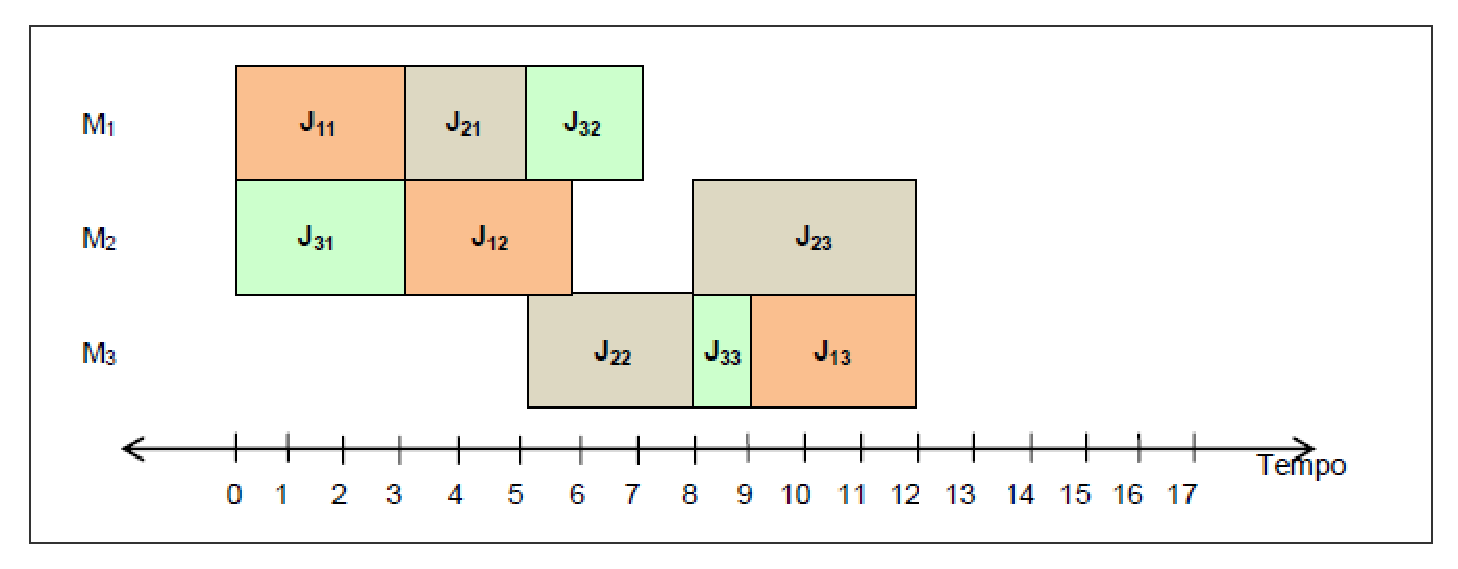
\includegraphics[scale = 0.6]{graficos/graf_gantt.eps}
\caption{Representação pelo Grafico de Gantt}
\label{graf_gantt}
\end{figure}

Nesse gráfico o eixo vertical representa as maquinas, o eixo horizontal representa a linha do tempo, e os retângulos representam as operações que compõem os Jobs, eles são encaixados no gráfico de modo que o seu tempo de execução fique marcado na linha do tempo. Os Jobs são identificados facilmente pela cor do retângulo, por exemplo, o Job 1 está representado pela cor laranja, onde $J_{11}$ representa a operação 1 do Job 1, o $J_{12}$ representa a operação 2 do Job 1 e o $J_{13}$ representa a operação 3 do Job 1. Com base na representação da solução da figura 1 o \textit{makespan}, ou seja, o tempo total de conclusão das operações é igual a 12 unidades de tempo.

\subsection{Grafos Disjuntivos}
Grafos Disjuntivos podem ser usados tanto para modelar um problema de \textit{Scheduling}, quanto para representar sua solução. A idéia principal dele consiste em mostrar a solução do problema destacando o uso das máquinas, e respeitando a precedência de operação dos Jobs. 

\subsubsection{Representação do Problema}
Um grafo parcialmente orientado, constituído por outros grafos pode ser usado como uma representação que reúne as características mais relevantes para o projeto de escalonamento de um problema de \textit{Job Shop Scheduling}. Uma representação do problema de \textit{Job Shop Scheduling} pode ser visualizada pelo Grafo Disjuntivo ilustrado na figura \ref{grafo_disjunt} 

\begin{figure}[H]
\centering
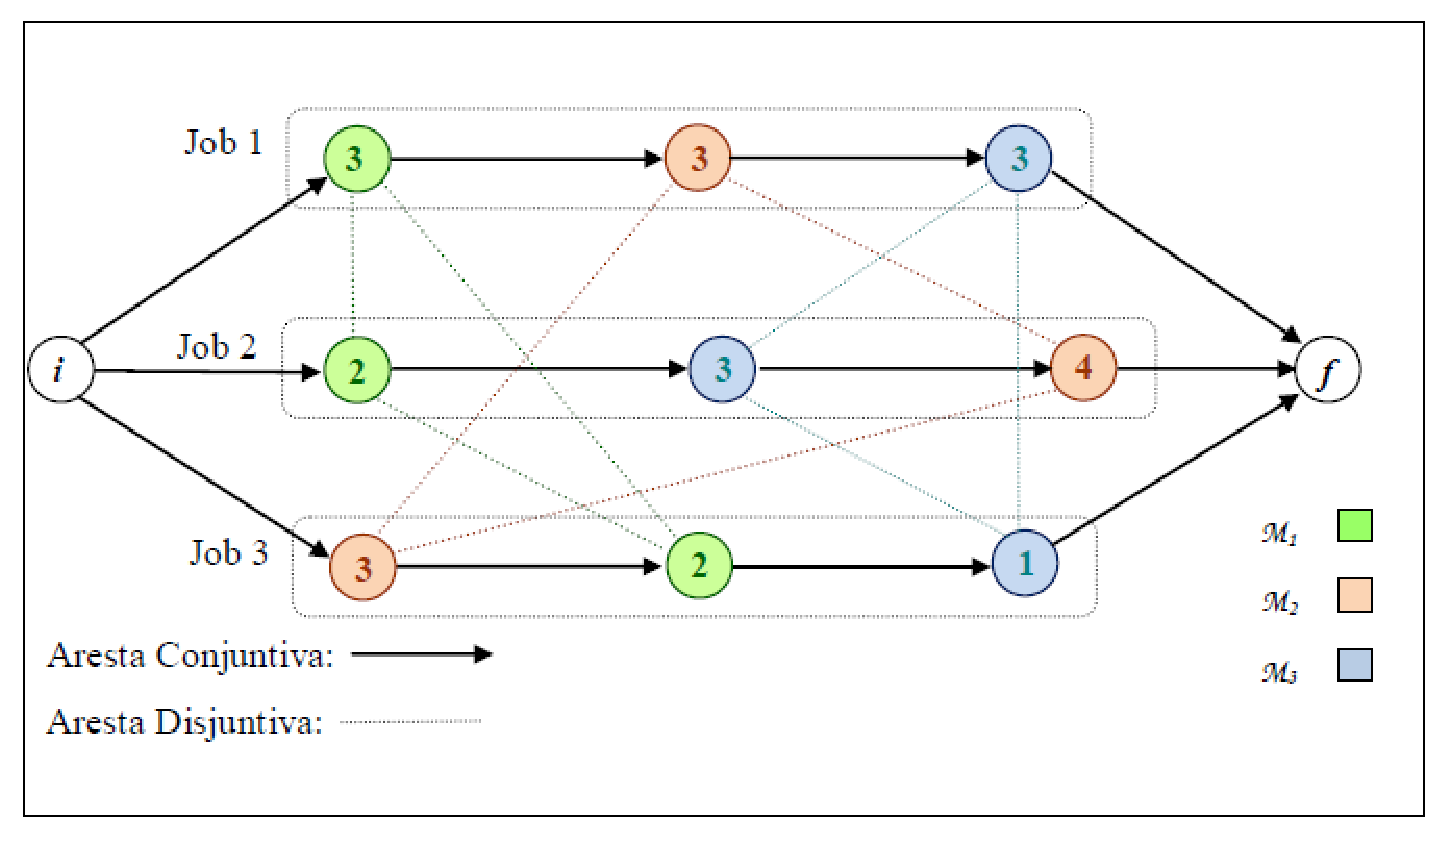
\includegraphics[scale = 0.6]{graficos/grafo_disjuntivo.eps}
\caption{Representação do problema usando grafo disjuntivo}
\label{grafo_disjunt}
\end{figure}

As operações de um mesmo Job estão interligadas por uma relação de dependência de prioridade de execução. Esta ligação é representada por arestas horizontais orientadas em um único sentido, as quais formam o grafo conjuntivo e elas não podem sofrer modificações de sentido. Cada operação deve ser executada por uma máquina diferente, as cores de cada job indica em qual máquina ele é executado, a interconexão não orientada forma o grafo disjuntivo, e relaciona os jobs que são executados pela mesma máquina, o número representado em cada operação na figura acima indica o tempo de processamento da operação.

\subsubsection{Representação da Solução}
Uma possível solução para o problema de Job Shop Scheduling pode ser representada por uma simples orientação do grafo disjuntivo, como mostra a Figura \ref{grafo_disj_orient}, lembrando que, somente as arestas disjuntivas podem sofrer modificações, pois elas indicam o escalonameto da máquina, e as arestas conjuntivas representam a restrição de precedência de operações.
	
Realizar um escalonamento das operações constituintes significa buscar uma solução para o problema, esse escalonamento das operações possui uma certa flexibilidade, pode ser alcançar diversas possibilidades de arranjo das operações, mas o grafo disjuntivo deve ser manter acíclico, pois uma operação só pode ser executada por uma máquina apenas uma vez.

\begin{figure}[H]
 \centering
 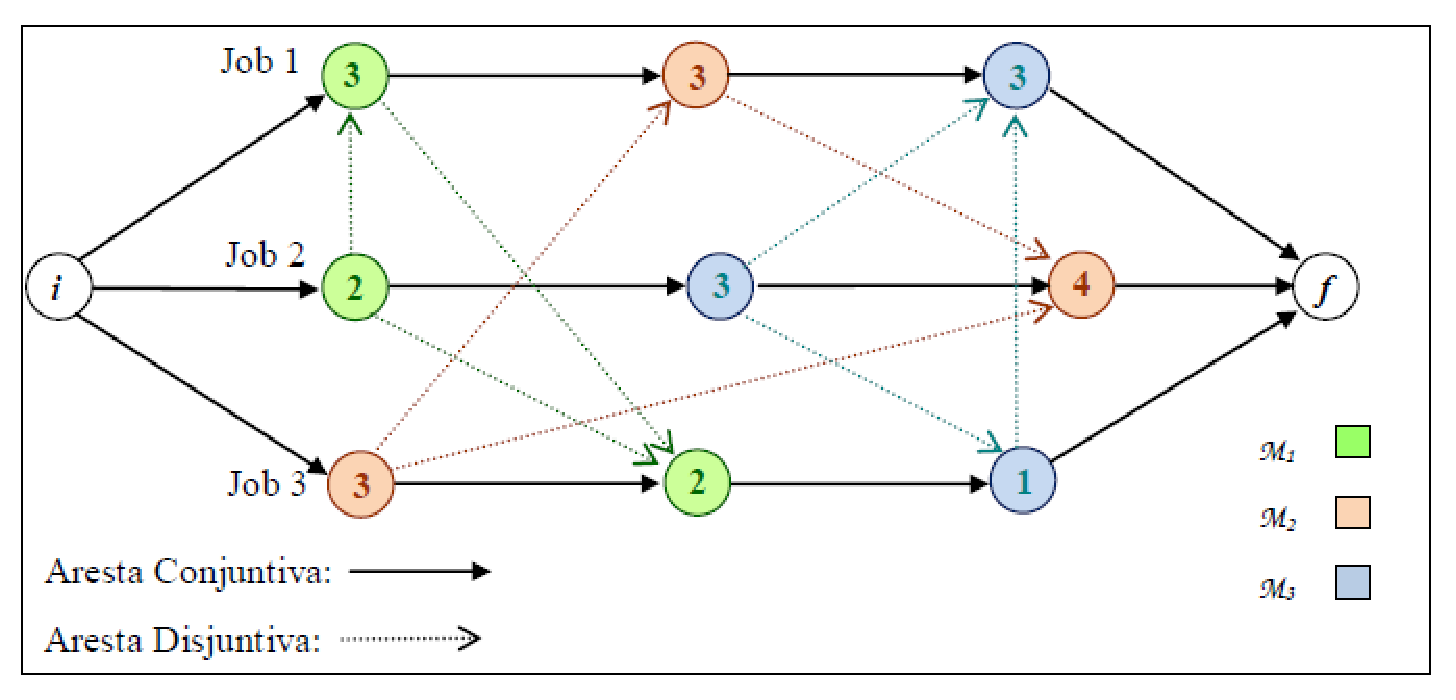
\includegraphics[scale = 0.6]{graficos/grafo_disjuntivo_orientado.eps}
 \caption{Representação da solução usando grafo disjuntivo orientado}
 \label{grafo_disj_orient}
\end{figure}

A solução encontrada através do escalonamento das operações no grafo disjuntivo necessita ser avaliada e comparada com outras soluções, uma forma de avaliação é analisar o tempo do caminho crítico, isto é, analisar o tempo de execução das operações mais demoradas \textcolor{red}{assim a solução encontrada deve ser menor que a análise do caminho crítico}.

\section{Métodos de Solução} \label{sec:met_sol}
O problema de \textit{Job Shop Scheduling} é classificado como NP-difícil, ou seja, é um problema para o qual não existem algoritmos que o resolva em tempo polinomial. Trata-se de um “Problema de Otimização Combinatória” \cite{SOUZA}.
Os algoritmos de solução podem ser classificados em duas classes:  Modelos matemáticos e Modelos heurísticos.

\begin{itemize}
\item \textbf{Modelos Matemáticos}: Trata-se de modelos de programação inteira mista, resolvidos pelos métodos branch and bound ou branch and cut.  Modelos Matemáticos enfatizam a obtenção de resultados ótimos em função de algum parâmetro de desempenho. Este pode ser, por exemplo, a minimização dos tempos de produção ou a maximização do uso dos recursos. Dependendo da complexidade do problema tratado, o calculo da solução ótima pode ser computacionalmente inviável.

\item \textbf{Modelos Heurísticos}: Trata-se de modelos baseados em regras pratica de escalonamento que enfatiza a obtenção de “boas” soluções, próxima da solução ótima. Os modelos heurísticos são caracterizados por obter uma solução aproximada em tempos de computação viáveis. 
\end{itemize}

\section{Heurística GRASP}
GRASP - {\it Greedy Randomized Adaptive Search Procedure}, ou procedimento de busca adaptativa gulosa e aleatória, é uma técnica iterativa proposta por \citeonline{FEO_REZENDE} que consiste numa fase de construção de uma solução viável, na qual uma solução é gerada, elemento a elemento, e de uma fase de busca local, na qual se procura melhorar de forma iterativa a qualidade da solução encontrada anteriormente, a fase de busca local trabalha de forma iterativa através de sucessivas substituições da solução atual por uma melhor de sua vizinhança, quando não há mais soluções melhores essa fase é terminada.

Na figura \ref{grasp}, encontra-se um pseudocógico genérico da heurística GRASP, os parâmetros que precisam ser definidos na heurísitca são o parâmetro de aleatoriedade $\alpha$ e o critério de parada (GRASPmax) que geralmente é o numero de iterações da heurística. De acordo com a figura \ref{grasp}, a heurística GRASP constrói repetidamente uma solução (passo 3) e esta é melhorada por uma busca local (passo 4) e a melhor solução encontrada até o momento é armazenada (passo 6 e 7).

A melhor solução encontrada ao longo de todas as interações GRASP realizadas é retornada como resultado do algoritmo de otimização GRASP \cite{SOUZA}

\begin{figure}[H]
\centering
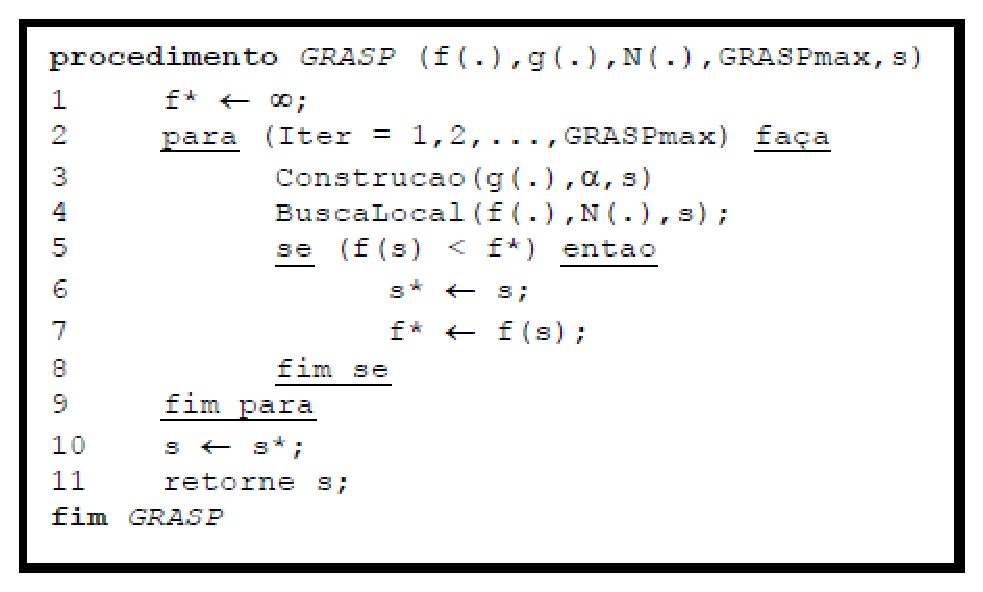
\includegraphics[scale = 0.8]{graficos/grasp.eps}  
\caption{Pseudo-código da heurística GRASP}

\label{grasp}
\end{figure}

Como o GRASP normalmente trata de problemas da ordem de complexidade NP-Dificil, poderia ficar indefinidamente em busca de uma solução ótima, para evitar esse caso, é preciso adotar um critério de parada na fase de busca local, por exemplo, o número máximo de iterações.

\subsection{Fase Construtiva}\label{teste}
Na fase de construção, uma solução é iterativamente construída, elemento por elemento. A cada iteração dessa fase, os próximos elementos candidatos a serem incluídos na solução são colocados em uma lista C de candidatos, seguindo um critério de ordenação pré-determinado. 

O processo de seleção é baseado em uma função adaptativa gulosa g : C → R , que estima o benefício da seleção de cada um dos elementos. A heurística é adaptativa porque os benefícios associados com a escolha de cada elemento são atualizados em cada iteração da fase de construção para refletir as mudanças oriundas da seleção do elemento anterior. A componente probabilística $\alpha$ $\in$ [0,1], denominada taxa gulosa, reside no fato de que cada elemento é selecionado de forma aleatória a partir de um subconjunto restrito formado pelos melhores elementos que compõem a lista de candidatos. Este subconjunto recebe o nome de lista de candidatos restrita LCR. Essa técnica de escolha permite que diferentes soluções sejam geradas em cada iteração GRASP.

O parâmetro $\alpha$ controla o nível de gulosidade e aleatoriedade na geração das soluções durante as iterações GRASP. Um valor $\alpha$ = 0 faz gerar soluções puramente gulosas, enquanto $\alpha$ = 1 faz produzir soluções totalmente aleatórias. 
As soluções geradas pela fase de construção do GRASP provavelmente não são localmente ótimas com respeito à definição de vizinhança que adotaremos a seguir na fase de busca local. Daí a importância da fase de busca local, a qual objetiva melhorar a solução construída.
	
O pseudocódigo da figura \ref{construction_phase} descreve a fase de construção da Solução GRASP.

\begin{figure}[H]
	\centering
	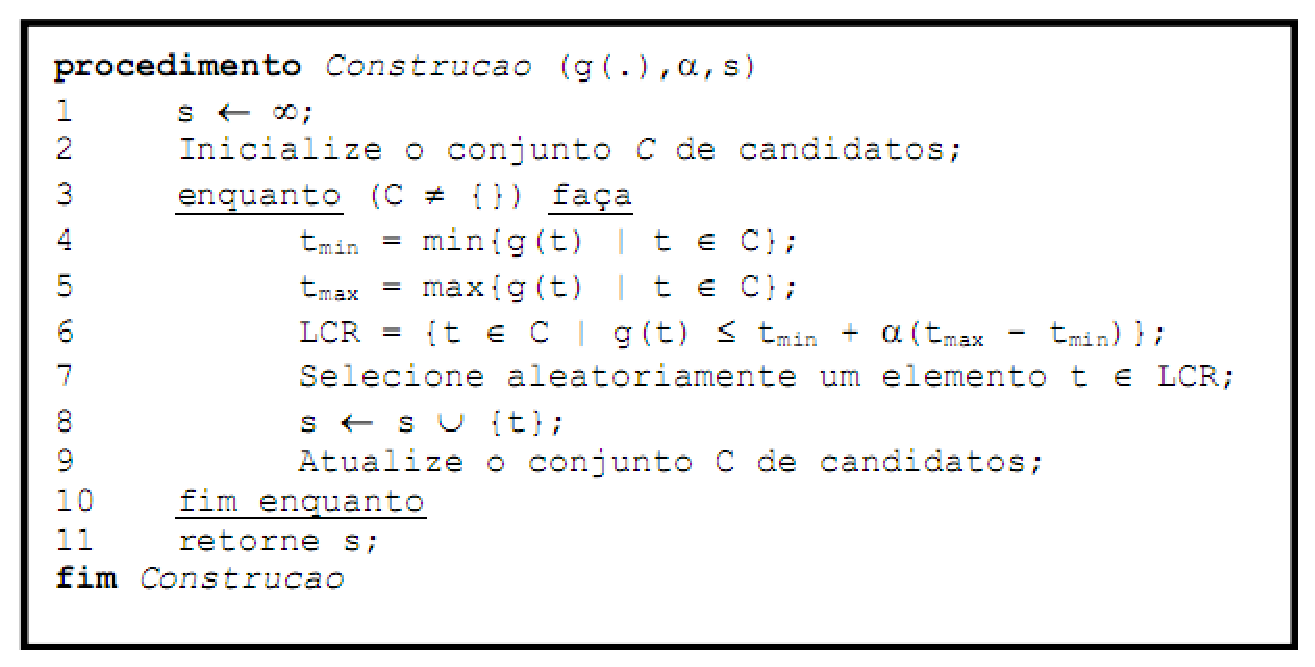
\includegraphics[scale=0.6]{graficos/grasp_construction_phase.eps}

	\caption{pseudo-código da fase de construção da heurística GRASP}
	\label{construction_phase}
\end{figure}

\subsection{Fase de Busca Local}
A fase de busca local está baseada na noção de vizinhança. A função N, a qual depende da estrutura do problema tratado, associa a cada solução viável s sua vizinhança N(s). Cada solução s' $\in$ N(s) é chamado de vizinho de s. É denominado movimento a modificação m que transforma uma solução s em outra s’, que esteja em sua vizinhança. Representa-se essa operação por s' $\leftarrow$ s $\in$ m. 
Em linhas gerais, a fase de busca local, começando de uma solução obtida pela fase de construção GRASP, navega pelo espaço de pesquisa passando de uma solução para outra, que seja sua vizinha, em busca de um ótimo local. 
A figura \ref{local_search_phase} descreve o pseudo-código de um algoritmo básico de busca local com respeito a uma certa vizinhança N(.) de s.

\begin{figure}[H]
	\centering
	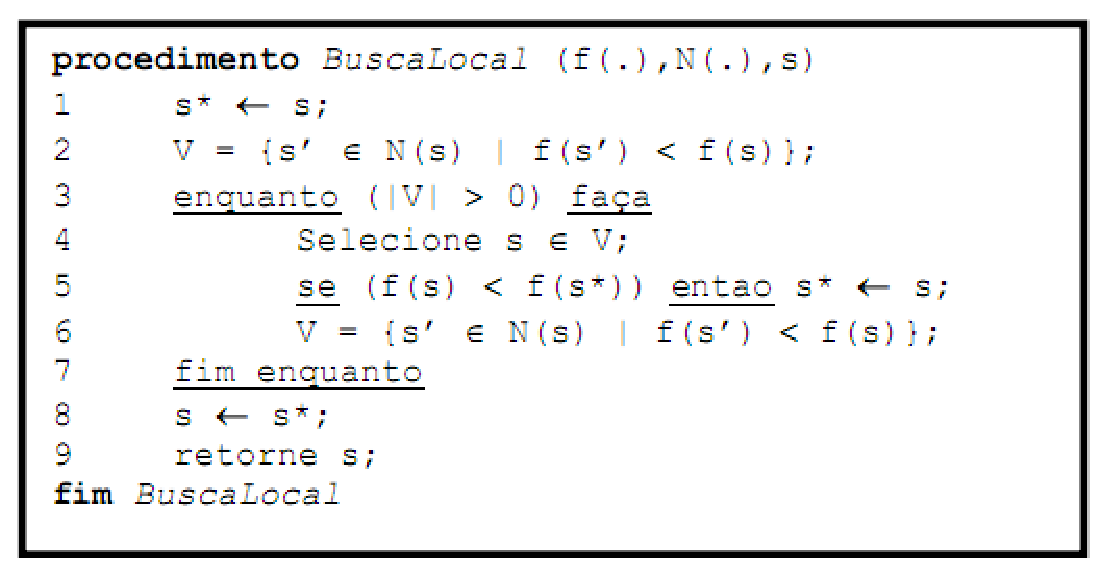
\includegraphics[scale=0.6]{graficos/grasp_local_search_phase.eps}
	\caption{pseudo-código da fase de busca local da heurística GRASP}
	\label{local_search_phase}
\end{figure}

\section{O problema de Sequenciamento de Tarefas e suas Aplicações}
A programação de tarefas constitui-se num alvo de pesquisa a ser buscado por fábricas de diversas designações, as quais disponham de máquinas destinadas a papéis específicos com o fim de produzir, comumente, mais de um tipo de produto e, às vezes, utilizando uma mesma máquina em alguma etapa do processo; com o objetivo de minimizar o tempo ocioso e maximizar a produtividade.

Embora o nome seqüenciamento de tarefas parece sugerir que o problema seja aplicado no ramo de produção industrial, ele ocorre em variados contextos, pode ser um ambiente de aplicação do problema, por exemplo, a distribuição de médicos e enfermeiros de um hospital, turmas e professores em uma sala de aula, navios em um porto, cidades e caxeiros viajantes, etc. \cite{REIS} 

% pseudocodigo com borda
%\begin{figure}[H]
%    \begin{center}
%       \begin{tabular}{c} \hline
%        \begin{lstlisting}[mathescape] 
%	${\bf procedimento}$ GRASP (f(.), g(.), N(.), GRASPmax, s)
%	$f^{*} \leftarrow \infty$;
%	para (iter = 1,2, ..., GRASPmax) faca
%		$\quad$Construcao(g(.), $\alpha$, s);
%		$\quad$BuscaLocal(f(.), N(.), s);
%		se (f(s) < $f^{*}$ entao
%			$\quad s^{*} \leftarrow s$;
%			$\quad f^{*} \leftarrow f(s)$;
%		fim se
%	fim para
%	s $\leftarrow s^{*}$;
%	retorne s;
%	fim GRASP
%	\end{lstlisting}\\
%\hline
% \end{tabular}
% \end{center}
%\caption{Pseudocode with a border}
%\label{fig-pseudocod-borderless}
%    \end{figure}


%\centering\begin{tabular}{c}\border
%\begin{lstlisting}[mathescape]
%Procedimento GRASP (f(.), g(.), N(.), GRASPmax, s)
%$f^{*} <-- \alpha$;
%\end{lstlisting}

%\end{tabular}




%Sinais de entrada provenientes de fora da rede chegam por meio de conexões
%originadas do mundo externo, de modo semelhante, saídas da rede para o mundo
%externo são conexões que deixam a rede.

%A configuração da rede, ou seja, os peso atual das conexões, determina como os
%dados de entrada irão ativar os diferentes neurônios e gerar um determinado
%resultado. Para grande maioria dos tipos de redes neurais, uma configuração
%particular é obtida através de um algoritmo de treinamento. O treinamento em
%geral busca reforçar as conexões que geram bons resultados e penalizar as que
%não geram.

%Estre as tarefas para as quais uma rede neural é adequada se
%incluem: classificação, reconhecimento de padrões, predições, otimização
%e filtragem de ruído.

%\section{Principais tipos de redes neurais}\label{sec:red_tip}

%Dentre a grande variedade de tipos de redes neurais artificiais, as mais
%importantes, seja por sua contribuição teórica ou pela praticidade, são:

%\subsection{Rede perceptron multicamada}

%A perceptron multicamada é (a) uma rede direta, isto é, o sinal passa da entrada
%até a saída sem ciclos; (b) possui camadas intermediárias de neurônios entre as
%camadas de entrada e saída, ditas camadas ocultas; (c) utiliza funções de
%ativação não lineares, comumente a função sigmoide e (d) os neurônios são
%altamente conectados, em geral cada neurônio é conectado a todos os neurônios
%da camada anterior e da camada seguinte.

%\begin{figure}[H]
%\centering

%\caption{Texto da figura}
%\end{figure}

%A presença de múltiplas camadas permite a este tipo de rede resolver uma enorme
%variedade de problemas, ou em outros termos, reconhecer uma vasta variedade de
%padrões. As redes multicamadas são computacionalmente completas, ou seja, são
%equivalentes à classe das máquinas de Turing.

%A retropropagação é o algoritmo de treinamento mais utilizado para esta variante
%de rede neural. Cada iteração deste algoritmo é dividido em dois passos, no
%primeiro a rede é alimentada com um dos exemplos, o resultado é capturado e
%comparado com o valor esperado, com isso o erro geral da rede é calculado;
%segue-se então ao segundo passo, que atualiza os pesos sinápticos penalizando
%cada neurônio segundo sua influência no erro geral, essa etapa é feita da camada
%de saída para a de entrada, retroativamente.

%\subsection{Rede de Hopfield}

%A rede de Hofield é (a) uma forma de rede neural recorrente, isto é,
%determinadas conexões realimentam alguns neurônios, formando ciclos na rede; (b)
%apresenta um atraso temporal, ou seja, a propagação dos sinais não é instantânea
%e (c) a saída é um estado de convergência, isto é, após se apresentar uma entrada
%a rede opera em ciclos até que a saída não mude mais, situação onde se diz que a
%rede alcançou o equilíbrio.

%ESQUEMA DE UMA REDE DE HOPFIELD AQUI

%A rede de Hopfield funciona como uma memória endereçada por conteúdo, ou memória
%associativa, por exemplo, muitas vezes lembramos de fatos inteiros apenas com uma
%pequena lembrança do acontecimento. Uma memória associativa é, deste modo, um
%conjunto de padrões armazenados de tal modo que, quando se apresenta um novo padrão,
%a resposta será o padrão armazenado que seja mais parecido a este que foi apresentado.

%Geralmente as redes de Hopfield não possuiem um método de aprendizado associado,
%os pesos sinápticos são calculados por métodos matemáticos provenientes de sua
%definição formal. A definição formal garante que a rede sempre irá convergir,
%contudo, em algumas situações esta convergência pode não ocorrer para o padrão
%mais próximo da entrada, e ainda não existe um método conhecido que resolva
%este problema.

%\subsection{Redes de Kohonen}

%As redes de Kohonen apresentam apenas duas camadas de neurônios, a camada de
%entrada e a de saída. A camada de saída é uma espécie de malha de neurônios não
%conectados entre si, mas amplamente conectados com os neurônios da camada de
%entrada. Esta malha funciona como um mapa, onde para cada padrão de entrada
%apenas um neurônio é ativado, padrões semelhantes ativam neurônios dentro de
%uma mesma região da malha.

%ESQUEMA DE UMA REDE DE KOHONEN AQUI

%As redes de Kohonen possuem um algoritmo próprio de treinamento, dividido em
%três etapas; na primeira, chamado de processo competitivo, uma determinada entrada
%ativa apenas um neurônio da malha; na segunda, chamado de processo cooperativo,
%o neurônio escolhido estabelece uma vizinhança de neurônios que serão ajustados
%para, junto com ele, identificar padrões semelhantes ao que foi apresentado; e
%por fim, na terceira etapa, chamada de processo adaptativo, os pesos são
%atualizados com base no neurônio vencedor e na vizinhança topológica. Este
%algoritmo de treinamento é dito não supervisionado, pois não depende de um
%par \textit{(entrada, saída esperada)}, já que a própria rede estabelece como
%será a configuração dos resultados.

%\section{Redes neurais de Kohonen}\label{sec:red_khn}

%Esta seção irá apresentar mais detalhadamente como é a configuração de uma rede
%de Kohonen, seu algoritmo de treinamento e os usos comuns deste tipo de rede.

%\subsection{Topologia de uma rede de Kohonen}

%Como dito anteriormente, a rede de Kohonen apresenta apenas duas camadas de
%neurônios, a camada de entrada e a camada de saída. A camada de entrada deve
%possuir tantos neurônios quanto forem à quantidade de elementos do padrão de
%entrada. A camada de saída é uma grade de geometria livre, geralmente
%retangular, de neurônios que não estão ligados entre si, mas estão, cada um,
%ligados a todos os neurônios da camada de entrada. As conexões apresentam pesos
%para escalar o sinal enviado.

%ESQUEMA DE UMA CONEXÃO DA REDE DE KOHONEN AQUI

%\subsection{Treinamento da rede}

%O treinamento requer que os pesos sinápticos sejam iniciados com valores bem
%pequenos, para que a rede não apresente inicialmente nenhuma configuração. Três
%processos são executados para cada entrada do conjunto de treinamento, o
%processo competitivo, o processo cooperativo e o processo adaptativo.

%\subsubsection{Processo competitivo}

%Quando uma entrada $ x = \left[x_1, x_2, ..., x_n\right]^T $ é apresentado à
%rede, o neurônio da grade que melhor responder a este padrão será ativado, este
%neurônio é dito vencedor, e será recompensado ajustando-se seus componentes
%para mais próximo do vetor de entrada.

%O critério escolhido para determinar o neurônio vencedor é a distância
%euclidiana entre o vetor de entradas e o vetor de pesos das sinapses do
%neurônio, como indicado na equação \ref{eq:dit_ecl}:

%\begin{equation}\label{eq:dit_ecl}
%d_i(t) = \sqrt{\sum_{j = 1}^N \left( x_j(t) - w_{ij}(t) \right)^2}
%\end{equation}

%Onde:

%\begin{itemize}
%\item $ d_i(t) $ é a distância euclidiana entre o vetor de pesos do
%neurônio $ i $ e o vetor de entradas na iteração $ t $;
%\item $ i $ é o índice do neurônio da grade;
%\item $ j $ é o índice do neurônio de entrada;
%\item $ N $ é o número de entradas;
%\item $ x_j(t) $ é o sinal de entrada na entrada $ j $ na iteração $ t $;
%\item $ w_{ij}(t) $ é o valor do peso sináptico entre o neurônio de
%entrada $ j $ e o neurônio da grade $ i $ na iteração $ t $.
%\end{itemize}

%\subsubsection{Processo cooperativo}

%Estudos biológicos indicam que ao ser excitado, um neurônio estimula seus
%vizinhos topológicos, de forma que quanto mais próximo um neurônio está do
%neurônio ativo, mais excitado pelo estímulo do neurônio ativo ele é. O processo
%cooperativo busca simular este mecanismo biológico.

%Em termos matemáticos, o que se deseja é um parâmetro $ h_{ik} $ , dito
%\textit{vizinhança topológica}, que indica o gral de cooperação entre o
%neurônio vencedor $ i $ e o seu vizinho $ k $, que deve ser simétrico em relação
%ao neurônio $ k $ e deve decrescer constantemente com o aumento da
%distância $ l_{ik} $ , até que $ \lim\limits_{ l_{ik} \to \infty } h_{ik} = 0 $ .
%A função gaussiana \ref{eq:gauss} atende a estas duas exigências:

%\begin{equation}\label{eq:gauss}
%h_{ik} = e^{ \left( \frac{ l_{ik}^2 }{ 2 \sigma^2 } \right) }
%\end{equation}

%O parâmetro $ \sigma $ é denominado \textit{largura efetiva da vizinhança},
%e deve diminuir a cada iteração, indicando uma tendência de especialização da
%rede. Neste trabalho o parâmetro $ \sigma $ é a equação \ref{eq:leg_eft}:

%\begin{equation}\label{eq:leg_eft}
%\sigma(t) = \sigma_0 e^{ t / \tau_l }
%\end{equation}

%Onde:

%\begin{itemize}
%\item $ \sigma_0 $ é o valor inicial de $ \sigma $;
%\item $ t $ é a iteração atual;
%\item $ \tau_l $ é uma constante de tempo.
%\end{itemize}

%\subsubsection{Processo adaptativo}

%O processo adaptativo atualiza os pesos sinápticos a cada iteração, levando em
%consideração o neurônio vencedor e a vizinhança topológica. O ajuste dos pesos
%deve decrescer com o tempo, para evitar que novos dados comprometam seriamente
%o conhecimento já adquirido, substituindo padrões já estabelecidos por novos.
%Algo semelhante ocorre com o cérebro humano, ao decorrer do envelhecimento o
%aprendizado vai se tornando mais difícil.

%O ajuste $ \Delta w_{ij} $ que a sinapse entre o neurônio de entrada $ i $ e
%um neurônio da malha $ j $ deve sofrer é expresso pela equação \ref{eq:ajus}:

%\begin{equation}\label{eq:ajus}
%\Delta w_{ij} = \eta(t) h_{ik}(t) (x_j - w_{ij})
%\end{equation}

%Onde $ h_{ik}(t) $ é o parâmetro vizinhança topológica na iteração $ t $ ,
%referente ao neurônio vencedor $ k $ . O
%parâmetro \textit{taxa de aprendizagem} $ \eta(t) $ é definido pela
%expressão \ref{eq:tx_aprd}:

%\begin{equation}\label{eq:tx_aprd}
%\eta(t) = \eta_0 e^{ t / \tau_l }, \eta_0 \in [0, 1]
%\end{equation}

%Onde $ \tau_l $ é uma constante de tempo.

%\subsubsection{Algoritmo geral de treinamento}

%O algoritmo \ref{alg:trei_khn} resume as três etapas anteriores e descreve
%todo o processo de treinamento de uma rede de Kohonen:
%%\clearpage

%\begin{algorithm}[H]
%\caption{Treinamento de uma rede de Kohonen}\label{alg:trei_khn}
%\SetAlgoRefName{alg:trei_khn}
%\Entrada{$ \sigma_0 $ , $ \tau_l $ , $ \eta_0 $ e o valor do \textit{erro} }
%\Inicio{
%  \Repita{distâncias auclidianas $ \le $ erro}{
%    Calcular a \textit{largura efetiva} $ \sigma(t) $\;
%    Calcular a \textit{vizinhança topológica} $ h $\;
%    Calcular a \textit{taxa de aprendizado} $ \eta(t) $\;
%    \ParaCada{conexão}{
%      Calcular $ \Delta w $\;
%      Ajustar o arco\;
%    }
%  }
%}
%\end{algorithm}

%\section{Descritores de Hu}\label{sec:desc_hu}

%Os descritores de Hu são um conjunto de sete momentos invariantes a rotação,
%translação e escala.

%O momento bidimensional de ordem $ (p+q) $ é dado pela
%equação \ref{eq:mm_bid_cont}:

%\begin{equation}\label{eq:mm_bid_cont}
%m_{pq} = \iint x^p y^q f(x, y) \mathrm{d}x \mathrm{d}y, p, q \in
%\end{equation}

%A equação num domínio discreto, pode ser reescrita na forma:

%\begin{equation}\label{eq:mm_bid_disc}
%m_{pq} = \sum_{x, y} x^p y^q f(x, y), p, q \in
%\end{equation}

%A massa total da função $ f(x, y) $ é determinado pelo
%momento $ m_{00} $, conforme a equação \ref{eq:mm_bid_m00}:

%\begin{equation}\label{eq:mm_bid_m00}
%m_{pq} = \sum_{x, y} f(x, y), p, q \in
%\end{equation}

%Existe um ponto no qual a aplicação pontual da massa total gera o mesmo momento
%que a massa distribuída, este ponto é dito centroide de $ f(x, y) $ e suas
%coordenadas $ x $ e $ y $ são dadas pela equação \ref{eq:ct_xy}:

%\begin{subequations}\label{eq:ct_xy}
%%\begin{align}
%    \bar{x} = \frac{1}{ m_{00} } \sum x f(x, y) = \frac{ m_{10} }{ m_{00} } \\
%    \bar{y} = \frac{1}{ m_{00} } \sum y f(x, y) = \frac{ m_{01} }{ m_{00} }
%\end{align}
%\end{subequations}

%O momento central é obtido se deslocando a imagem para o centroide,
%da seguinte forma:

%\begin{equation}\label{eq:mm_ctr}
%\mu_{pq} = \sum_{x, y} (x - \bar{x})^p (y - \bar{y})^q f(x, y)
%\end{equation}

%Ainda é necessário normalizar o momento para que os valores resultantes não sejam
%extremos a ponto de serem ignorados pelo sistema de reconhecimento de padrões. O
%momento central de ordem $ (p+q) $ normalizado é obtido dividindo o momento
%central de $ y $ mesma ordem por um fator definido por $ \mu_{00}^\gamma $ ,
%conforme indicado pela equação \ref{eq:mm_norm}:

%\begin{subequations}\label{eq:mm_norm}
%\begin{align}
%    \gamma = 1 + \frac{ p + q }{2} \\
%    \eta_{pq} = \frac{ \mu_{pq} }{ \mu_{00}^\gamma }
%\end{align}
%\end{subequations}

%A partir dessas equações são estabelecidos sete momentos invariantes à translação,
% rotação e escala, chamados de momentos de Hu, ou descritores de Hu. São eles:

%\begin{subequations}\label{eq:mmt}
%\begin{align}
%  \varphi_1 = \eta_{20} + \eta_{02} \\
%  \varphi_2 = (\eta_{20} - \eta_{02})^2 + 4\eta_{11}^2 \\
%  \varphi_3 = (\eta_{30} - 3\eta_{12})^2 + (3\eta_{21} - \eta_{03})^2 \\
%  \varphi_4 = (\eta_{30} + \eta_{12})^2 + (3\eta_{21} + \eta_{03})^2 \\
%%
%  \varphi_5 = (\eta_{30} - 3\eta_{12})(\eta_{30} + \eta_{12})
%               \left[ (\eta_{30} + \eta_{12})^2 - 3(\eta_{21} + \eta_{03})^2 \right] \\
%              + (3\eta_{21} - \eta_{03})(\eta_{21} + \eta_{03})
%               \left[ 3(\eta_{30} + \eta_{12})^2 - (\eta_{21} + \eta_{03})^2 \right] \\
%%
%  \varphi_6 = (\eta_{20} - \eta_{02})
%               \left[ (\eta_{30} + \eta_{12})^2 - (\eta_{21} + \eta_{03})^2 \right] \\
%              + 4\eta_{11}(\eta_{30} - \eta_{12})(\eta_{21} + \eta_{03}) \\
%%
%  \varphi_7 = (3\eta_{21} - \eta_{30})(\eta_{30} + \eta_{12})
%               \left[ (\eta_{30} + \eta_{12})^2 - 3(\eta_{21} + \eta_{03})^2 \right] \\
%              + (3\eta_{12} - \eta_{03})(\eta_{21} + \eta_{03})
%               \left[ 3(\eta_{30} + \eta_{12})^2 - (\eta_{21} + \eta_{03})^2 \right]
%\end{align}
%\end{subequations}

%\section{Imagens digitais}\label{sec:img_dig}

%Imagens digitais são representações computacionais de imagens bidimensionais,
%codificadas de modo a permitir seu armazenamento, exibição e manipulação por
%dispositivos eletrônicos. Há dois tipos fundamentais de imagens digitais,
%os mapas de bits (\textit{bitmaps}) e as imagens vetoriais.

%\subsection{Mapas de bits}

%Mapa de bists é a representação matricial de uma imagem, onde cada posição,
%chamada de \textit{pixel}, armazena uma cor. Normalmente os \textit{pixels} são
%codificados no padrão RGB (\textit{Red}, \textit{Green},\textit{Blue}), que
%utiliza três \textit{bytes} para armazenar um inteiro para as cores vermelha,
%verde e azul, respectivamente. Em mídias impressas é comum que as imagens
%\textit{bitmaps} utilizem o padrão
%CMYK (\textit{Cian}, \textit{Magenta}, \textit{Yelow}, \textit{	Black}) ao invés
%do RGB.

%Embora uma imagem bitmap seja armazenada na RAM com todos os \textit{pixels}, é
%comum, por uma questão de economia de memória e tempo de transmissão, a compressão
%destes arquivos. Entre os principais formatos de compressão estão
%o GIF (\textit{Graphics Interchange Format}), o JPEG
%(\textit{Joint Photographic Experts Group}) e o PNG (\textit{Portable Network Graphics}).

%\subsection{Imagens vetoriais}

%As imagens vetoriais são formadas pela descrição geométrica de objetos.
%Por serem compostas de vetores, este tipo de imagem ocupa menos espaço na
%memória comparado com as bitmaps, e não perdem a qualidade quando
%aplicado transformações de escala e rotação sobre elas.

